\chapter{Elgendiho referenční algoritmus}
\label{chap:elgendi_neurokit}
% Úvod do tématu - odkud co bereme, proč to děláme, co je cílem
Tato kapitola popisuje, jak lze ve fotopletysmografickém (\acs{PPG}) signálu nalézt systolické vrcholy s využitím Elgendiho algoritmu, který je implementován v~knihovně NeuroKit2.

Tato knihovna reaguje na \uv{krizi reprodukovatelnosti}, což je problém, kdy vědecké studie nelze opakovaně potvrdit kvůli nedostupnosti kódu a dat.
Proto nabízí otevřený zdrojový kód, strukturovanou dokumentaci i podporu k začleňování funkcí přímo do výzkumných prací~\cite{NeuroKit2}.
Zdrojový kód pro NeuroKit2 je dostupný na \url{https://github.com/neuropsychology/NeuroKit} a dokumentace na \url{https://neurokit2.readthedocs.io/}.
Knihovnu je možné průběžně modifikovat a vyvíjet.

V~kapitole~\ref{chap:PPG_teorie} byly již podrobně shrnuty principy \acs{PPG}, proto se zde zaměříme na samotnou detekci vrcholů a její realizaci.

\section{Obecná struktura algoritmu}
\label{sec:alg_structure}
% základní popis - co dělá, jaké jsou vstupy a výstupy, obrázek
Algoritmus se skládá z několika kroků: \emph{filtrace} pomocí pásmové propusti, \emph{umocnění} signálu, vytvoření dvou \emph{klouzavých průměrů} a dvou \emph{prahů} (Obr.~\ref{fig:alg-scheme})~\cite{Elgendi2013}.
Vstupem je surový fotopletysmografický záznam, zatímco výstupem jsou konkrétní časové pozice nalezených systolických vrcholů.

\begin{figure}[h]
	\centering
	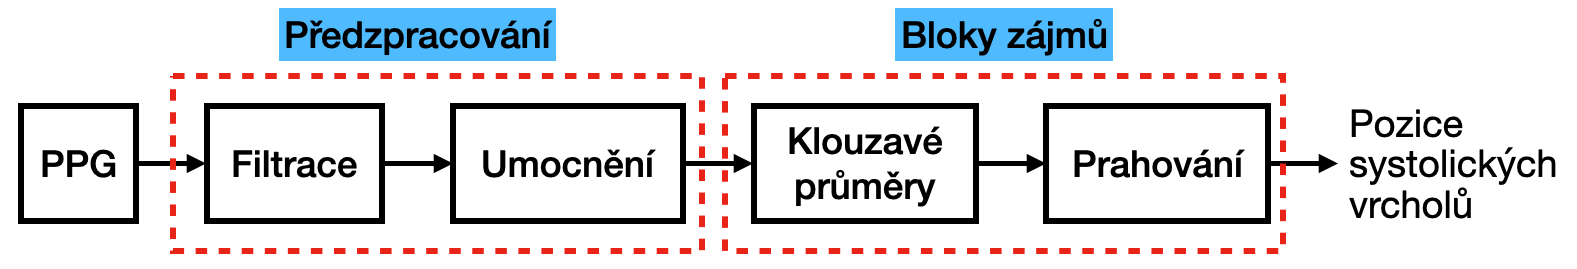
\includegraphics[width=1\textwidth]{./obrazky/ElgendiBlokSchema.png}
	\vspace{-5mm}
	\caption[Struktura Elgendiho algoritmu]{Zjednodušené schéma Elgendiho algoritmu~\cite{Elgendi2013}.}
	\vspace{-5mm}
	\label{fig:alg-scheme}
\end{figure}

\section{Předzpracování signálu}
\label{sec:preprocess}
% Filtrace - butterworthův filtr PP
% Kolísání nulové izolinie = baseline wander (https://dspace.vut.cz/server/api/core/bitstreams/8172d61c-ba8b-4edb-a2eb-2cebccbdc952/content)
% Umocnění - jen kladné hodnoty, zbytek nula
% KEEP IN MIND: Nepotlačují se frekvence, ale složky o vyšších/nižších frekvencích.
\begin{figure}[!t]
	\centering
	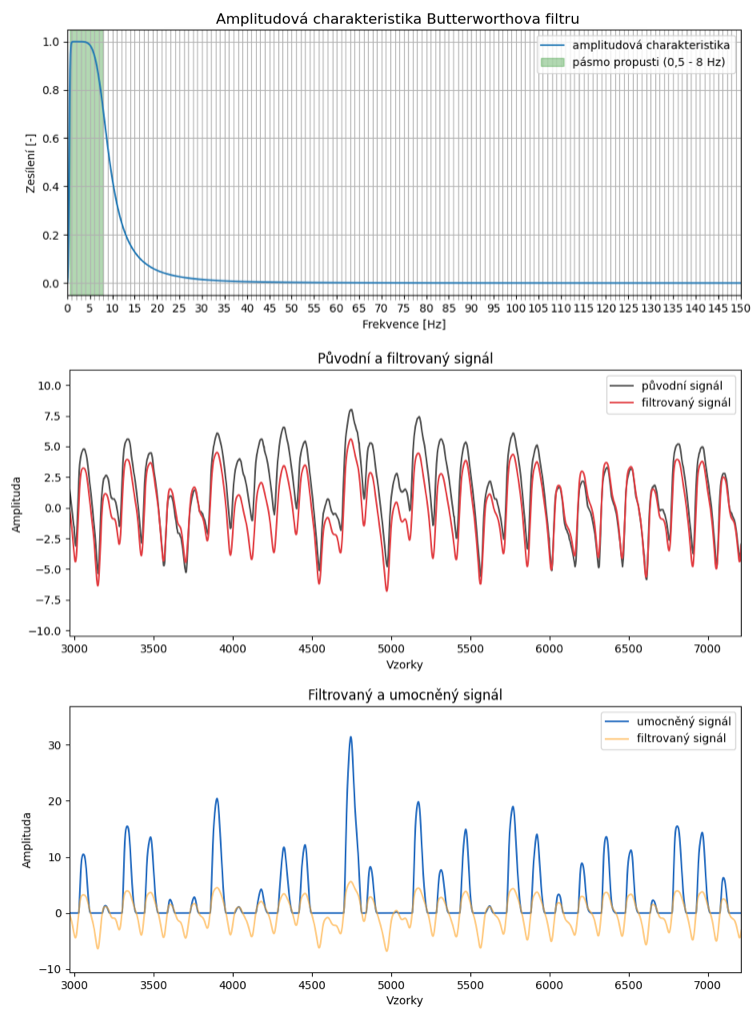
\includegraphics[width=1\textwidth]{./obrazky/ElgendiAFC_PP_Sq.png}
	\caption[Elgendiho předzpracování PPG signálu]{Filtrace PPG signálu pomocí Butterworthova filtru a umocnění.}
	\label{fig:filter-example}
\end{figure}

Pro samotnou detekci vrcholů připraví Elgendi~\cite{Elgendi2013} signál pomocí filtrace a umocnění kladných hodnot.
Elgendi používá Butterworthův filtr druhého řádu, který je zpracován v~přímém i reverzním směru (tzv.~filtrace s nulovým fázovým posuvem), ale v knihovně NeuroKit2 je implementován filtr třetího řádu.
My jsme se rozhodli přenastavit funkci v knihovně tak, aby odpovídala původnímu filtru druhého řádu, což je náš jediný zásah do kódu knihovny.
Filtr je nastaven jako pásmová propust s~dolní a horní mezí 0,5~Hz a 8~Hz, který má potlačit ty složky signálu, které odpovídají šumu a kolísání nulové izolinie~\cite{Elgendi2013}.
Na Obr.~\ref{fig:filter-example} je ukázka amplitudové charakteristiky filtru a porovnání původního a filtrovaného úseku signálu.

Po filtraci je kaldná část signálu umocněna na druhou viz.~(\ref{eq:square}).
To je provedeno s cílem zdůraznit rozdíly mezi systolickou vlnou a ostatními složkami, jako jsou diastolické zářezy nebo šum~\cite{Elgendi2013}.
Výsledná hodnota $y[n]$ po umocnění je dána vztahem:
\begin{equation}
	\label{eq:square}
		y[n] =
		\begin{cases}
			Z[n]^2, & \text{pokud } Z[n] > 0,\\[1mm]
			0, & \text{pokud } Z[n] \le 0.
		\end{cases}
	\end{equation}
kde $Z[n]$ představuje již vyfiltrovaný signál.
Porovnání filtrovaného a umocněného signálu je ilustrováno na Obr.~\ref{fig:filter-example}.

\section{Určení bloků zájmů a nalezení vrcholů}
\label{sec:thr_peaks}
% 
Po úvodní filtraci a umocnění fotopletysmografického signálu, vypočítává Elgendiho algoritmus dva klouzavé průměry (\acs{MA}), které se od sebe liší v samotné šířce průměrujícího okna~\cite{Elgendi2013}.

Kratší okno \(W_1\) je nastaveno tak, aby sloužilo ke zdůraznění systolické špičky, zatímco delší okno \(W_2\) se vybralo tak, aby zdůraznilo období celého srdečního cyklu.
Tyto konstanty odpovídají šířkám oken v milisekundách, ve kterých se počítají klouzavé průměry (\ref{eq:MA_P}) a (\ref{eq:MA_B}).
Pro vypočítání konkrétních velikostí oken bylo provedeno metodou \uv{hrubé sily} vhodných parametrů tak, že se vyzkoušely různé kombinace délek těchto a dalších a konstant.
Jako nejlepší kombinace se vybrala ta, po které dosahoval algoritmus nejvyššího skóre v citlivosti (\acs{Se}) a pozitivní prediktivní hodnotě (\acs{PPV}) na trénovací sadě dat~\cite{Elgendi2013}.
Pro \(W_1\) byla zvolena hodnota 111 (odpovídající milisekundám) a pro \(W_2\) hodnota 667.

\subsection*{Výpočet klouzavých průměrů} % ⚠️ Lépe popsat = porozumět + dodat graf
\label{sec:MA}
% 
Elgendi definuje umocěný a vyfiltrovaný \acs{PPG} signál jako \(y[n]\).
Klouzavý průměr s kratším oknem \acs{MA_P} se pro každý bod \(n\) vypočítá rovnicí

\begin{equation}
	MA_{peak}[n] \;=\;
	\frac{1}{W_1}
	(y[n - \frac{W_1-1}{2}] + \ldots + y[n] + \ldots + y[n + \frac{W_1-1}{2}]),
	\label{eq:MA_P}
\end{equation}

kde je \(W_1\) konstanta popsaná v podkapitole~\ref{sec:thr_peaks}~\cite{Elgendi2013}
Podobně se s delším oknem \(W_2\) vypočítá \acs{MA_B}, který reprezentuje přibližnou délku jednoho srdečního cyklu:

\begin{equation}
	MA_{beat}[n] \;=\;
	\frac{1}{W_2}
	(y[n - \frac{W_2-1}{2}] + \ldots + y[n] + \ldots + y[n + \frac{W_2-1}{2}]).
	\label{eq:MA_B}
\end{equation}

Výsledky výpočtů jsou zobrazeny na Obr.~\ref{fig:thresholds_peaks_clean} a Obr.~\ref{fig:thresholds_peaks}.
Tyto klouzavé průměry slouží k vypočítání \acs{THR_1} a následných bloků zájmu, které vedou k~určení systolických vrcholů.

\subsection*{Nastavení dvou dynamických prahů}
\label{sec:thresholds}
% 
Pro další zpracování se zvolí dvě prahové hodnoty.
První dynamický práh \acs{THR_1} se vpočítá posunutím signálu \acs{MA_B} o konstantu \(\beta\) vynásobenou průměrnou hodnotou umocněného signálu \(\overline{z}\) viz.~(\ref{eq:THR_1}).
Tato průměrná hodnota se vypočítává z celého umocněného signálu.
\(\beta\) je jedním z~parametrů, který se nastavuje metodou \uv{hrubé síly} a nejlepší výsledky vyšly, když se \(\beta\) nastavila na hodnotu 2~\cite{Elgendi2013}.

\begin{equation}
	THR_1[n] \;=\; MA_{beat}[n] \;+\; \beta \,\cdot\, \overline{z}.
	\label{eq:THR_1}
\end{equation}

První práh je vykreslen na Obr.~\ref{fig:thresholds_peaks_clean} a Obr.~\ref{fig:thresholds_peaks} společně s klouzavými průměry a umocněným signálem.
Z těchto obrázků je patrné, že parametry \(\beta\) ani \(\overline{z}\) nemají na práh \acs{THR_1} příliš významný viditelný efekt, tudíž je křivka \acs{THR_1} velmi podobná křivce \acs{MA_B}.

Porovnáním \acs{MA_P}[n] s~\acs{THR_1}[n] získáme časové úseky (tzv. bloky zájmu), které odpovídají částem, kde je signál nad úrovní \acs{MA_B}.

Druhý práh \acs{THR_2} slouží k pročištění již stanovených bloků zájmů a je roven konstantě \(W_1\).
Elgendi využívá tento práh pro eliminaci všech bloků, které jsou kratší než předem stanovená konstanta reprezentující očekávanou šířku systolické vlny~\cite{Elgendi2013}.

\subsection*{Určení bloků zájmů}
\label{sec:blocks}
% ...
Porovnáním výše uvedeného klouzavého průměru \acs{MA_P} a prvního prahu (\acs{THR_1}) jsou určeny bloky zájmu.
Tyto bloky jsou definovány jako úseky, kde je \acs{MA_P} větší než \acs{THR_1} a zároveň jejich šířka je větší než \acs{THR_2} viz.~(\ref{eq:blocks})~\cite{Elgendi2013}.
Bloky zájmu jsou zobrazeny jako šedé úseky na Obr.~\ref{fig:thresholds_peaks_clean} a~\ref{fig:thresholds_peaks}.

\begin{equation}
	\{n : MA_{peak}[n] > THR_1[n] \; \land \; okno > THR_2\}.
	\label{eq:blocks}
\end{equation}

Na Obr.~\ref{fig:thresholds_peaks} vidíme tři systolické vrcholy, které nebyly detekovány (kolem vzorků 4000, 4600 a 5000).
U prvního z nich je patrné, že umocněný signál překračuje \acs{THR_1}, avšak blok je příliš krátký, a proto je vyřazen.
Druhý a třetí vrchol mají ve filtrovaném signálu příliš nízkou amplitudu, což způsobuje, že po umocnění nejsou dostatečně výrazné.

\subsection*{Nalezení vrcholů}
\label{sec:peaks}

Samotné systolické vrcholy jsou určeny jako lokální maxima v~oblastech bloků zájmu.
Funkce \(find\_peaks\) z~knihovny NeuroKit2 zpracovává jednodimenzionální signál a porovnáváním hodnot v~každém bloku zájmu určuje lokální maxima~\cite{NeuroKit2}.

\begin{figure}[t]
	\vspace{-9mm}
	\centering
	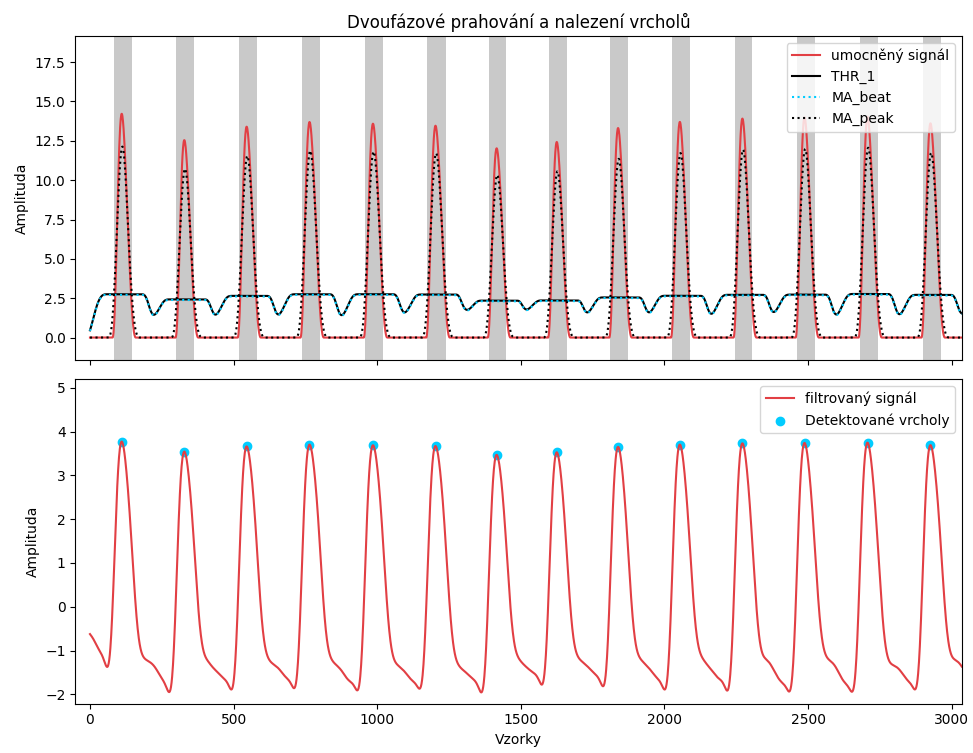
\includegraphics[width=1\textwidth]{./obrazky/Elgendi_THR_Peaks_Clean.png}
	\vspace{-10mm}
	\caption[Elgendiho zpracování pravidelného signálu]{Nastavení bloků zájmu a určení systolických vrcholů pro pravidelný signál.}
	\label{fig:thresholds_peaks_clean}
\end{figure}

\begin{figure}[b]
	\centering
	\vspace{-10mm}
	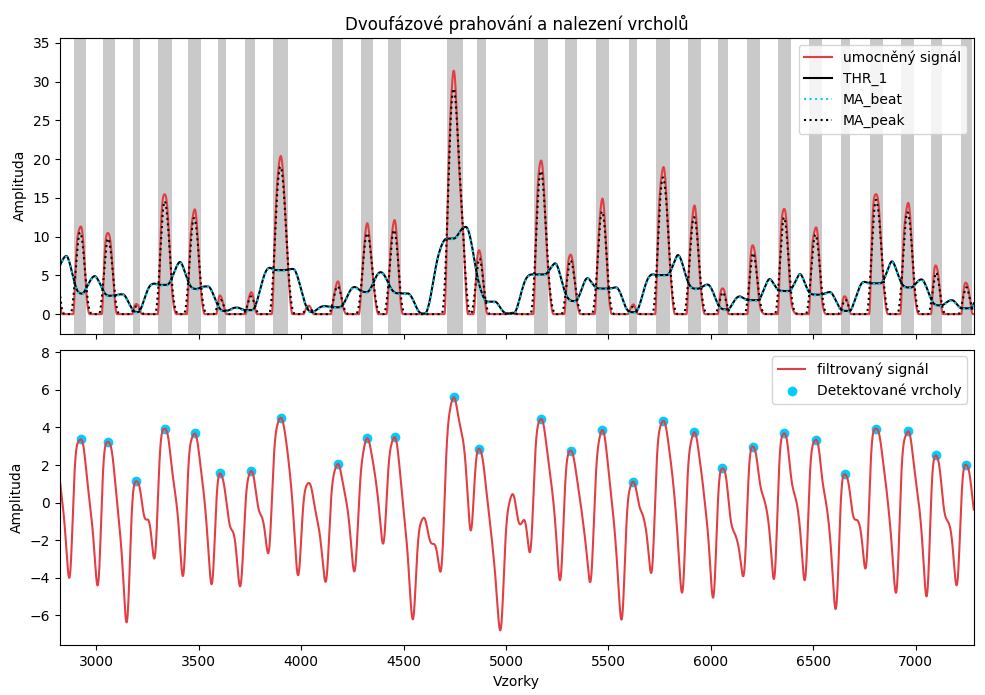
\includegraphics[width=1\textwidth]{./obrazky/Elgendi_THR_Peaks.png}
	\caption[Elgendiho zpracování nepravidelného signálu]{Nastavení bloků zájmu a určení systolických vrcholů pro nepravidelný signál.}
	\vspace{-15mm}
	\label{fig:thresholds_peaks}
\end{figure}